\section{Transfer of Thermal Energy}

\textbf{Conduction} is\\
\textbf{Convection} is \\
\textbf{Radiation} is

\begin{multicols}{2}


\subsection{Football Model of Thermal Energy}

\begin{center}
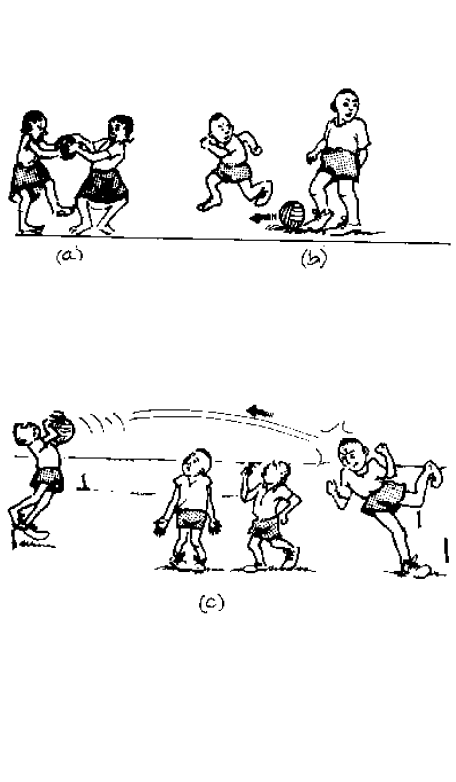
\includegraphics[width=0.4\textwidth]{./img/source/football-thermal.png}
\end{center}

\begin{description*}
%\item[Subtopic:]{}
\item[Materials:]{}
\item[Setup:]{}
\item[Procedure:]{}
\item[Hazards:]{}
\item[Questions:]{}
\item[Observations:]{}
\item[Theory:]{}
\item[Applications:]{}
\item[Notes:]{}
\end{description*}

\subsection{Heat Transfer in a Candle}

\begin{center}
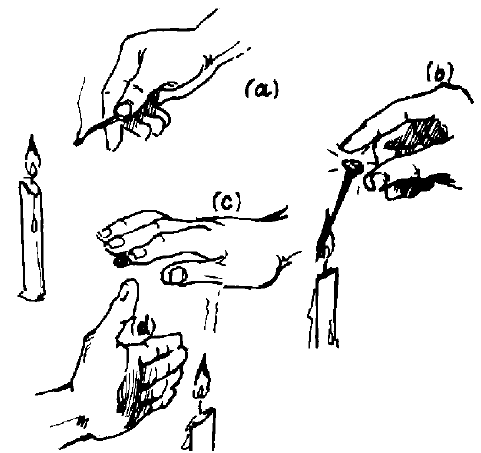
\includegraphics[width=0.4\textwidth]{./img/source/heat-trans-candle.png}
\end{center}

\begin{description*}
%\item[Subtopic:]{}
\item[Materials:]{}
\item[Setup:]{}
\item[Procedure:]{}
\item[Hazards:]{}
\item[Questions:]{}
\item[Observations:]{}
\item[Theory:]{}
\item[Applications:]{}
\item[Notes:]{}
\end{description*}

%==================================================================================================%

\section*{Conduction}


\subsection{Good and Bad Conductors of Heat}

\begin{center}
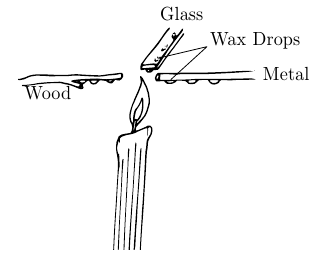
\includegraphics[width=0.4\textwidth]{./img/heat-conduction.png}
\end{center}

\begin{description*}
%\item[Subtopic:]{}
\item[Materials:]{}
\item[Setup:]{}
\item[Procedure:]{}
\item[Hazards:]{}
\item[Questions:]{}
\item[Observations:]{}
\item[Theory:]{}
\item[Applications:]{Cooking pots are made of metal to efficiently transfer heat to the food. \emph{Insulators} are poor conductors of heat and are used to prevent heat loss (e.g. in clothes).}
\item[Notes:]{}
\end{description*}

\subsection{Rate of Conduction}

\begin{center}
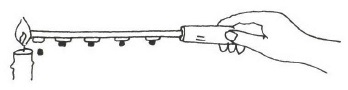
\includegraphics[width=0.4\textwidth]{./img/vso/conduction-rate.png}
\end{center}

\begin{description*}
%\item[Subtopic:]{}
\item[Materials:]{}
\item[Setup:]{}
\item[Procedure:]{}
\item[Hazards:]{}
\item[Questions:]{}
\item[Observations:]{}
\item[Theory:]{}
\item[Applications:]{}
\item[Notes:]{}
\end{description*}

\subsection{Coin Burn}

\begin{center}
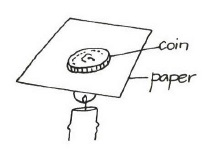
\includegraphics[width=0.4\textwidth]{./img/vso/coin-burn.png}
\end{center}

\begin{description*}
%\item[Subtopic:]{}
\item[Materials:]{}
\item[Setup:]{}
\item[Procedure:]{}
\item[Hazards:]{}
\item[Questions:]{}
\item[Observations:]{}
\item[Theory:]{}
\item[Applications:]{}
\item[Notes:]{}
\end{description*}

\subsection{Paper Pan}

\begin{center}
\includegraphics[width=0.4\textwidth]{./img/vso/paper-burn.png}
\end{center}

\begin{description*}
%\item[Subtopic:]{}
\item[Materials:]{}
\item[Setup:]{}
\item[Procedure:]{}
\item[Hazards:]{}
\item[Questions:]{}
\item[Observations:]{}
\item[Theory:]{}
\item[Applications:]{}
\item[Notes:]{}
\end{description*}

\subsection{Fireproof Material}

\begin{center}
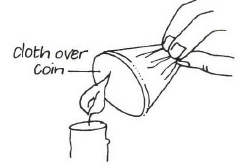
\includegraphics[width=0.4\textwidth]{./img/vso/fireproof.png}
\end{center}

\begin{description*}
%\item[Subtopic:]{}
\item[Materials:]{}
\item[Setup:]{}
\item[Procedure:]{}
\item[Hazards:]{}
\item[Questions:]{}
\item[Observations:]{}
\item[Theory:]{}
\item[Applications:]{}
\item[Notes:]{}
\end{description*}

\subsection{Candle Snuffer}

%\begin{center}
%\includegraphics[width=0.4\textwidth]{./img/source/.png}
%\end{center}

\begin{description*}
%\item[Subtopic:]{}
\item[Materials:]{}
\item[Setup:]{}
\item[Procedure:]{}
\item[Hazards:]{}
\item[Questions:]{}
\item[Observations:]{}
\item[Theory:]{}
\item[Applications:]{}
\item[Notes:]{}
\end{description*}

%==================================================================================================%

\section*{Convection}


\subsection{Convection Detectors}

\begin{center}
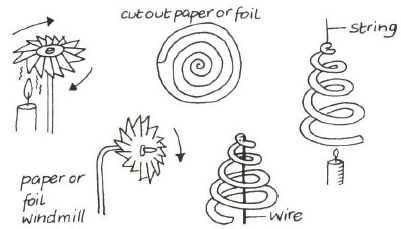
\includegraphics[width=0.4\textwidth]{./img/vso/convection-detectors.png}
\end{center}

\begin{description*}
%\item[Subtopic:]{}
\item[Materials:]{}
\item[Setup:]{}
\item[Procedure:]{}
\item[Hazards:]{}
\item[Questions:]{}
\item[Observations:]{}
\item[Theory:]{}
\item[Applications:]{}
\item[Notes:]{}
\end{description*}


\subsection{Convection Currents}

\begin{center}
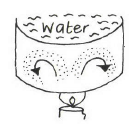
\includegraphics[width=0.4\textwidth]{./img/vso/convection-currents.png}
\end{center}

\begin{description*}
%\item[Subtopic:]{}
\item[Materials:]{}
\item[Setup:]{}
\item[Procedure:]{}
\item[Hazards:]{}
\item[Questions:]{}
\item[Observations:]{}
\item[Theory:]{}
\item[Applications:]{}
\item[Notes:]{}
\end{description*}

\subsection{Breeze as a Convection Current}

\begin{center}
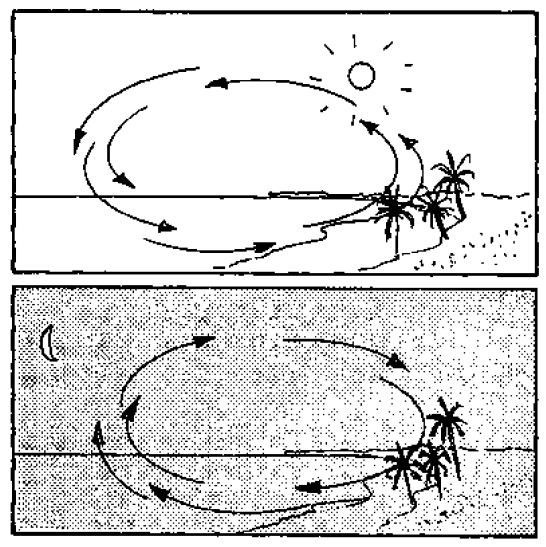
\includegraphics[width=0.4\textwidth]{./img/source/breeze.png}
\end{center}

\begin{description*}
%\item[Subtopic:]{}
\item[Materials:]{}
\item[Setup:]{}
\item[Procedure:]{}
\item[Hazards:]{}
\item[Questions:]{}
\item[Observations:]{}
\item[Theory:]{}
\item[Applications:]{}
\item[Notes:]{}
\end{description*}

\subsection{Ventilation System}

\begin{center}
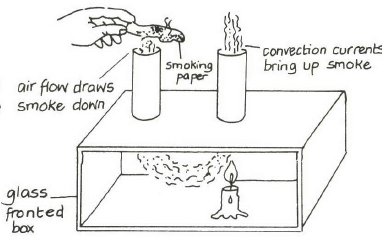
\includegraphics[width=0.4\textwidth]{./img/vso/ventilation-system.png}
\end{center}

\begin{description*}
%\item[Subtopic:]{}
\item[Materials:]{}
\item[Setup:]{}
\item[Procedure:]{}
\item[Hazards:]{}
\item[Questions:]{}
\item[Observations:]{}
\item[Theory:]{}
\item[Applications:]{}
\item[Notes:]{}
\end{description*}

\subsection{Hot Air Balloon}

\begin{center}
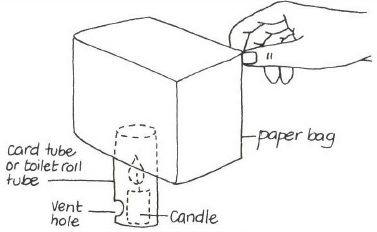
\includegraphics[width=0.4\textwidth]{./img/vso/hot-air-balloon.png}
\end{center}

\begin{description*}
%\item[Subtopic:]{}
\item[Materials:]{}
\item[Setup:]{}
\item[Procedure:]{}
\item[Hazards:]{}
\item[Questions:]{}
\item[Observations:]{}
\item[Theory:]{}
\item[Applications:]{}
\item[Notes:]{}
\end{description*}

%==================================================================================================%

\section*{Radiation}


\subsection{Good and Bad Radiators}

\begin{center}
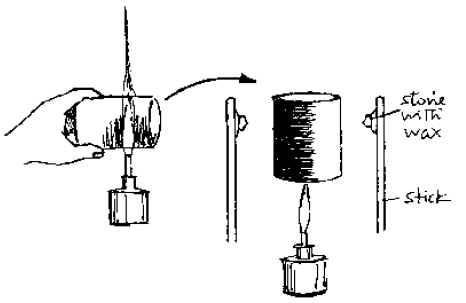
\includegraphics[width=0.4\textwidth]{./img/source/good-bad-radiators.png}
\end{center}

\begin{description*}
%\item[Subtopic:]{}
\item[Materials:]{}
\item[Setup:]{}
\item[Procedure:]{}
\item[Hazards:]{}
\item[Questions:]{}
\item[Observations:]{}
\item[Theory:]{}
\item[Applications:]{}
\item[Notes:]{}
\end{description*}

\subsection{Good and Bad Heat Absorbers}

\begin{center}
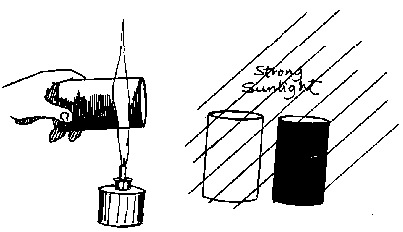
\includegraphics[width=0.4\textwidth]{./img/source/good-bad-absorbers.png}
\end{center}

\begin{description*}
%\item[Subtopic:]{}
\item[Materials:]{}
\item[Setup:]{}
\item[Procedure:]{}
\item[Hazards:]{}
\item[Questions:]{}
\item[Observations:]{}
\item[Theory:]{}
\item[Applications:]{}
\item[Notes:]{}
\end{description*}

%==================================================================================================%


\end{multicols}

\pagebreak